%%%%%%
%
% $Autor: Wings $
% $Datum: 2020-01-18 11:15:45Z $
% $Pfad: githubtemplate/Template/Presentations/Template/slides/rename.tex $
% $Version: 4620 $
%
%
% !TeX encoding = utf8
% !TeX root = Rename
%
%%%%%%



\Mysection{Trajectory Planning}

\STANDARD{Trajectory Planning}
{ 
	
  \framesubtitle{Einleitung}	
  
  \begin{figure}[!h]
    \centering
    \begin{tikzpicture}

\draw  (-3,0.5) node[left] (v1) {$q_0=q(t_0)$} ellipse (0.05 and 0.05);
\draw  (-0.5,2.5) node[right] (v2) {$q_1=q(t_1)$} ellipse (0.05 and 0.05);
\draw[-latex]  (-3,0.5) -- node[above,left]{$q=q(t)$} (-0.5,2.5);
\end{tikzpicture}
  \end{figure}

  Wir müssen hier unterscheiden zwischen:

  \begin{itemize}
    \item der Beschreibung der Position der Aktoren
    \item und der Beschreibung der Lage des Effektors (Werkzeugs)
      \begin{itemize}
        \item diese wird auch als Pose bezeichnet und kann durch 3 Positionsangaben (wie x,y,z) und 3 Drehwinkel (wie a,b,c) bezogen auf ein Bezugskoordinatensystem beschrieben werden
%Weber, Industrieroboter Seite 16 
        \item sie beschreibt eine Bahn im Raum
      \end{itemize}
  \end{itemize}

  \textbf{Einschränkung}: zunächst nur die Position der Aktoren
}


\STANDARD{Trajectory Planning}
{ 

  \textbf{Aufgabe}: Beziehung zwischen Zeit und Position finden

  \textbf{Synonyme}: Path Planning, Motion Planning

  Unterscheidung hier:

  \begin{itemize}
    \item Geometrie (Path): Position der Aktoren ohne Zeitinformation
    \item Trajektorie (Trajectory): Position, Geschwindigkeit, Beschleunigung und Ruck als Funktion über die Zeit
  \end{itemize}
% Seite 2 Trajectory generation for a four axis robot with linear kinematics - S.N. van den Brink - DCT 2005.69
%With a trajectory we indicate the position, velocity, acceleration and jerk profiles of every actuator as a function of time.
%With a path, the subsequent positions of every actuator without time information is indicated

\textbf{Vereinfachung}

  \begin{itemize}
    \item Eindimensionale Trajektorie: $q=q(t)$
          \\Definiert durch eine Skalar-Funktion
    \item Mehrdimensionale Trajektorie: $\textbf{p}=\textbf{p}(t)$
          \\Definiert durch eine Vektor-Funktion
  \end{itemize}

  \textbf{Einschränkung}: zunächst nur eindimensionale Trajektorien; \cite{Piegl:1997}
}

\STANDARD{Trajectory Planning}
{ 

  $q_0$: Startposition

  $q_1$: Zielposition

  \begin{figure}[!h]
    \centering
    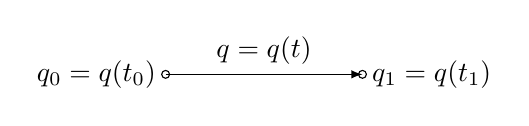
\begin{tikzpicture}

\draw  (-3,0.5) node[left] (v1) {$q_0=q(t_0)$} ellipse (0.05 and 0.05);
\draw  (-0.5,0.5) node[right] (v2) {$q_1=q(t_1)$} ellipse (0.05 and 0.05);
\draw[-latex]  (-3,0.5) -- node[above]{$q=q(t)$} (-0.5,0.5);
\end{tikzpicture}
  \end{figure}
}

\section{Notation}
\STANDARD{Notation}
{ 


  Position

  \begin{equation}
    q(t)
  \end{equation}

  Geschwindigkeit (Velocity)

  \begin{equation}
    v(t) 
    = \dot{q}(t) 
    = \frac{d}{dt} q(t)
  \end{equation}

  Beschleunigung (Acceleration)

  \begin{eqnarray}
    a(t) 
    = \dot{v}(t) = \frac{d}{dt} v(t) 
    = \ddot{q}(t) = \frac{d^2}{dt^2} q(t)
  \end{eqnarray}

  Ruck (Jerk)

  \begin{eqnarray}
    j(t) 
    = \dot{a}(t) = \frac{d}{dt} a(t)
    = \ddot{v}(t) = \frac{d^2}{dt^2} v(t)
    = q^{(3)}(t) = \frac{d^3}{dt^3} q(t)
    %= \dddot{q}(t) = \frac{d^3}{dt^3} q(t)
  \end{eqnarray}
}


\section{Bang-Bang-Control}

\STANDARD{Bang-Bang-Control}
{ 

  \textbf{Prozess}: Positionierung

  \textbf{Aufgabe}: Positionieren in möglichst kurzer Zeit

  \textbf{Ansatz}: Höchstmögliches ausreizen der limitierende(n) Größe(n)

  \textbf{Grenzen}: Limitierende Größen (Constraints) ergeben sich

  \begin{itemize}
    \item durch den Motor
          
          über die Höchstdrehzahl wird $v_{max}$ festgelegt
          
          über das Drehmoment wird $a_{max}$ festgelegt
    \item durch die Dynamik des mechanischen Systems
          
          über Steifigkeit/Nachgiebigkeit wird $j_{max}$ festgelegt
    \item durch die Geometrie wird festgelegt, ob
          
          $j_{max}$, $a_{max}$ und $v_{max}$ überhaupt erreicht werden können
      \begin{itemize}
        \item da \textbf{hier} nur eindimensionale Trajektorien betrachtet werden, ist nur die \textbf{Weglänge} der begrenzende Faktor
        \item bei mehrdimensionalen Trajektorien ist die Krümmung ein weiterer begrenzender Faktor
      \end{itemize}
  \end{itemize}
}

\STANDARD{Water Taxi}
{
  \begin{center}
    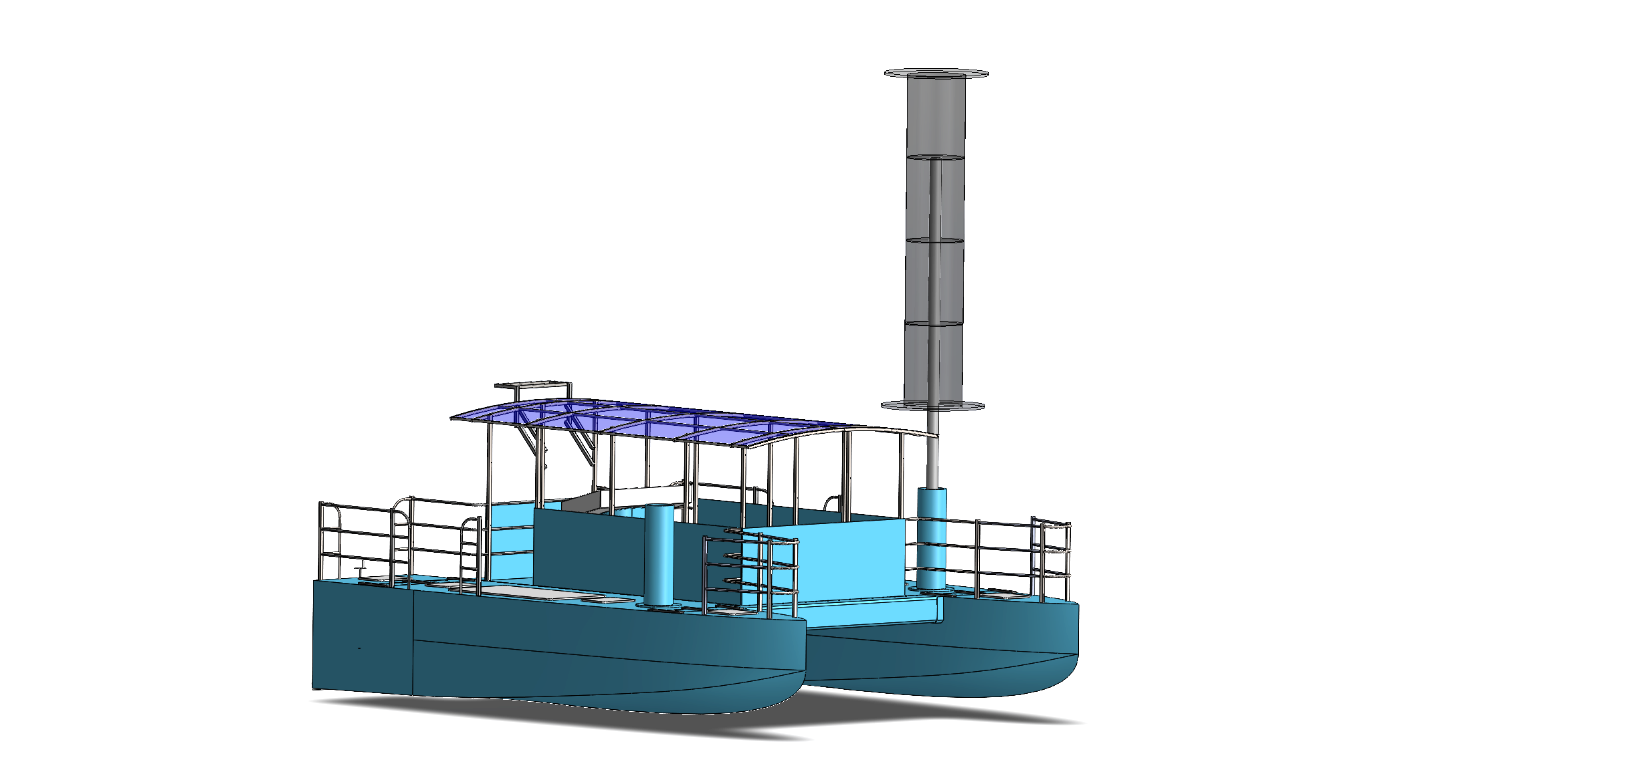
\includegraphics[width=\textwidth]{images/WaterTaxi}
  \end{center}	
}

\STANDARD{3D-Printer}
{
	\begin{center}
		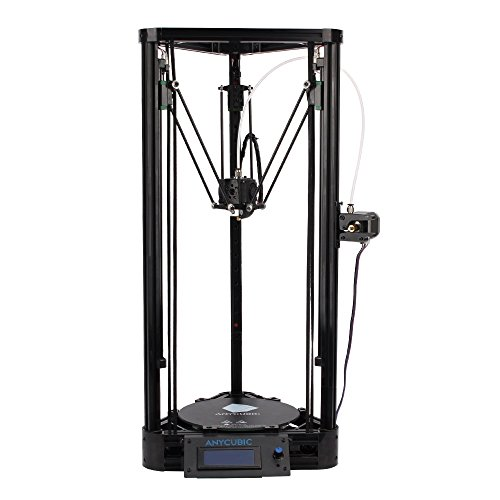
\includegraphics[height=0.8\textheight]{images/Rostock}
	\end{center}	
}


\STANDARD{3D-Printer}
{
  Der Datenstruktur \PYTHON{MyStructure} aus der Datei \FILE{MyStructure.py} ist sehr interessant.	
}


\begin{frame}[fragile]{Code}

%, numbers=left, caption={Konstruktion eines Keras-Sequential-Modells}, label={src:kerasmodel}]

  \begin{lstlisting}[language=Python]
import tensorflow as tf
from tensorflow.keras import datasets, layers, models

MODEL = models.Sequential()
  \end{lstlisting}

\end{frame}

\begin{frame}[fragile]{Code}

  \lstinputlisting[language=Python, firstnumber=1]{Code/PDFExtractTable/PDFExtractTable.py}
\end{frame}
